\chapter{Trabalhos Relacionados}
\label{cap:trabalhos}
Este capítulo apresenta os trabalhos relacionados ao objeto de pesquisa, obtidos por meio de um mapeamento sistemático da literatura. O objetivo desse mapeamento foi identificar, analisar e sintetizar estudos acadêmicos que abordam comparações entre as abordagens de renderização \acrshort{csr} (Client-Side Rendering) e \acrshort{ssr} (Server-Side Rendering) no contexto do desenvolvimento de aplicações web. Buscou-se compreender como essas estratégias impactam aspectos como desempenho, tempo de carregamento, \acrshort{seo}, experiência do usuário e escalabilidade. O protocolo adotado, descrito nas seções seguintes, foi elaborado para garantir a abrangência, a precisão e a relevância dos resultados encontrados.


\section{Questões de pesquisa}
\label{section:questoes_pesquisa}
\begin{enumerate}
    \item[Q1:] De que maneira a escolha entre \acrshort{csr} e \acrshort{ssr} influenciam a experiência do usuário?
    \item[Q2:] Como as abordagens \acrshort{csr} e \acrshort{ssr} afetam métricas de performance, tempo de carregamento e tempo até a interatividade em aplicações web?
    \item[Q3:] Quais são os principais desafios e \english{trade-offs} na implementação de \acrshort{csr} e \acrshort{ssr}?
    \item[Q4:] Quais trabalhos relacionados existem na literatura que abordam recomendações sobre quando usar o \acrshort{csr} ou \acrshort{ssr}?

\end{enumerate}

\section{Estratégia de busca}
Esta seção apresenta a estratégia de buscas de artigos científicos e livros relacionados à pesquisa. As ferramentas utilizadas para realizar as buscas são:
\begin{itemize}
    \item \textbf{Periódicos Capes:} É uma ferramenta disponibilizada pelo governo federal para uso de estudantes e pesquisadores. Acessando através da instituição de ensino ou pesquisa, é possível ter acesso completo a uma grande quantidade de artigos científicos publicados em variadas revistas, conferências e universidades. A principal vantagem dessa ferramenta é a possibilidade de ler o conteúdo integral de grande parte das publicações disponíveis. Por outro lado, as expressões de busca atualmente suportadas são bem limitadas.
    \item \textbf{\english{Scopus:}} Trata-se de um ferramenta similar ao Periódicos Capes. No entanto, o \english{Scopus} permite a elaboração de expressões de buscas mais complexas e sofisticadas, servindo para descobrir publicações não detectadas pelas outras plataformas. Além disso, possui um acervo bem mais amplo que o Periódicos Capes. Entretanto, algumas publicações não podem ser vistas na íntegra de forma gratuita.
    \item \textbf{\english{PICOC}}: A técnica \english{PICOC} foi utilizada para estruturar e refinar a estratégia de busca. Essa abordagem consiste em definir cinco elementos principais que auxiliam na formulação da expressão booleana para a pesquisa:
\begin{itemize}
    \item \textbf{P (População/Problema):} Define os estudos ou o grupo de interesse, ou seja, o problema ou a população que se deseja investigar. Por exemplo, “artigos que tratem da integração de tecnologias digitais na educação.”
    \item \textbf{I (Intervenção/Interesse):} Refere-se à intervenção, prática ou fenômeno que está sendo analisado. Neste caso, pode ser a “inserção de tecnologias digitais nos processos de ensino e aprendizagem.”
    \item \textbf{C (Comparação):} Descreve o(s) elemento(s) com os quais a intervenção ou situação é comparada, como “ensino tradicional” ou a comparação entre diferentes estratégias digitais, quando aplicável.
    \item \textbf{O (Outcome/Desfecho):} Indica os resultados ou efeitos esperados da intervenção. Por exemplo, “melhora do desempenho acadêmico” ou “maior engajamento dos alunos.”
    \item \textbf{C (Contexto):} Considera o ambiente ou cenário onde a intervenção ocorre, como “instituições de ensino, universidades” ou “publicações indexadas em bases internacionais.”
\end{itemize}
A partir da definição desses elementos, foi possível construir uma expressão booleana que unisse os principais termos de interesse para a pesquisa. Esse método colaborou para refinar os resultados, tornando a busca mais precisa e abrangente, conforme exemplificado no \autoref{quad:quadro_picoc}.
    \item \textbf{\english{Google Docs:}} Ferramenta desenvolvida pela \english{Google LLC} que permite a criação e edição de documentos de texto. Suas grandes vantagens em relação a ferramentas de outros fornecedores são as avançadas ferramentas de colaboração e a possibilidade de acesso por meio de navegadores \english{web}, sem necessidade de instalação de \english{software} específico.
    \item \textbf{\english{Google Sheets}}: Com as mesmas características e vantagens do \english{Google Docs}, essa ferramenta fornece recursos para elaboração de planilhas de cálculo. É muito útil para realizar análise de dados simples e também visualizar e apresentar dados tabulares.
\end{itemize}



% Como grande parte das publicações na área de computação são em inglês, esta pesquisa utiliza esse idioma para fazer buscas nas ferramentas indicadas. Além disso, \acrfull{csr} e \acrfull{ssr} são relativamente recentes, as buscas se limitaram a publicações feitas nos últimos 20 anos.

% Os termos-chave para realização das buscas são: Microsserviço, \acrshort{csr} e \acrlong{ssr}. Como a busca é feita em inglês, se usará \english{web performance} nas buscas.

\section{Quadro PICOC}
\label{section:quadro_picoc}

\begin{quadro}[H]
\centering

\setlength{\tabcolsep}{0.8em} % espaçamento horizontal
\renewcommand{\arraystretch}{1.5} % espaçamento vertical
\caption{Estrutura PICOC aplicada à pesquisa}
\begin{tabular}{|p{1.5in}|p{4.2in}|}
\hline
\textbf{Elemento} & \textbf{Descrição} \\ \hline

\textbf{P (População/Problema)} & 
Equipes de desenvolvimento web, arquitetos de software e gestores de TI que precisam escolher estratégias de renderização (\acrshort{csr} ou \acrshort{ssr}) para aplicações web modernas, visando otimizar desempenho, \acrshort{seo} e experiência do usuário. 
\\ \hline

\textbf{I (Intervenção)} & 
Adoção de técnicas de \textbf{\acrshort{csr}} (Client-Side Rendering): todo (ou quase todo) o conteúdo gerado no lado do cliente, utilizando frameworks/libraries como React, Vue, Angular etc.
\\ \hline

\textbf{C (Comparação)} & 
Implementação de \textbf{\acrshort{ssr}} (Server-Side Rendering): conteúdo pré-renderizado no servidor antes de ser enviado ao cliente, usando \emph{meta-frameworks} como Next.js, Nuxt.js, SvelteKit, Angular Universal, entre outros.
\\ \hline

\textbf{O (Outcome / Resultado)} & 
\begin{itemize}
  \item Métricas de desempenho (tempo de carregamento, \textit{time-to-first-byte}, \textit{largest contentful paint}, etc.)
  \item Impacto no \textbf{\acrshort{seo}} (indexabilidade, posicionamento em buscadores)
  \item Experiência do usuário e usabilidade
  \item Escalabilidade do sistema (uso de recursos de servidor/cliente)
\end{itemize}
\\ \hline

\textbf{C (Contexto)} & 
Aplicações web modernas que buscam equilibrar interatividade, rapidez de carregamento, otimização para motores de busca e redução de custos operacionais. O estudo pode ser aplicado a sistemas de e-commerce, portais de conteúdo, \emph{landing pages}, etc.
\\ \hline

\end{tabular}
\label{quad:quadro_picoc}
\fonte{os autores}
\end{quadro}


\subsection{Expressão de busca}
\label{section:string_busca}

\begin{quadro}[H]
\centering

\setlength{\tabcolsep}{0.8em} % for the horizontal padding
\renewcommand{\arraystretch}{1.5}% for the vertical padding
\caption{Expressão de busca utilizada}
\begin{tabular}{|p{4.5in}|}

\hline
Expressão de Busca \\ \hline
\english{(TITLE-ABS-KEY("Client-Side Rendering" OR "CSR" OR "Server-Side Rendering" OR "SSR")) AND (TITLE-ABS-KEY("web performance" OR "page speed" OR "web optimization" OR "SEO" OR "search engine optimization" OR "user experience" OR "UX" OR "usability"))} \\ \hline

\end{tabular}
\label{quad:string_busca}
\fonte{os autores}
\end{quadro}

\section{Estratégia de seleção}
\label{section:estrategia_selecao}
A estratégia de seleção dos artigos foi baseada em critérios de inclusão e exclusão, conforme descrito a seguir:
\begin{itemize}
    \item \textbf{Critérios de inclusão:}
    \begin{itemize}
        \item Artigos publicados entre 2020 e 2025.
        \item Artigos que abordem o impacto de \acrshort{csr} e \acrshort{ssr} em aplicações web.
        \item Artigos que apresentem resultados de experimentos ou estudos de caso relacionados a \acrshort{csr} e \acrshort{ssr}.
    \end{itemize}
    \item \textbf{Critérios de exclusão:}
    \begin{itemize}
        \item Artigos que não estejam disponíveis na íntegra.
        \item Artigos que não abordem diretamente o tema da pesquisa.
        \item Artigos que sejam duplicados ou muito semelhantes a outros já selecionados.
    \end{itemize}
\end{itemize}

\section{Caracterização de pesquisa}
\label{section:caracterizacao_pesquisa}
Na \autoref{fig:docs_by_year}, é apresentado o número de publicações identificadas por ano, no intervalo entre 2020 e 2025. Observa-se um crescimento progressivo de 2020 a 2023, culminando em um pico em 2023, com 15 documentos publicados. A partir desse ponto, nota-se uma queda significativa: em 2024, o número de publicações cai para 9, e em 2025 esse número se reduz ainda mais, atingindo apenas 3 documentos. Essa redução pode ser parcialmente atribuída ao fato de que a coleta foi realizada no mês de abril de 2025, o que possivelmente não contempla todas as publicações previstas para o ano. No total, foram encontrados 50 documentos relevantes, distribuídos de forma desigual, evidenciando uma tendência crescente de interesse pelo tema até 2023, seguido de uma possível estabilização ou atraso na indexação dos dados mais recentes.

\begin{figure}[H]
    \centering
    \caption{Número de publicações ao longo dos anos}
    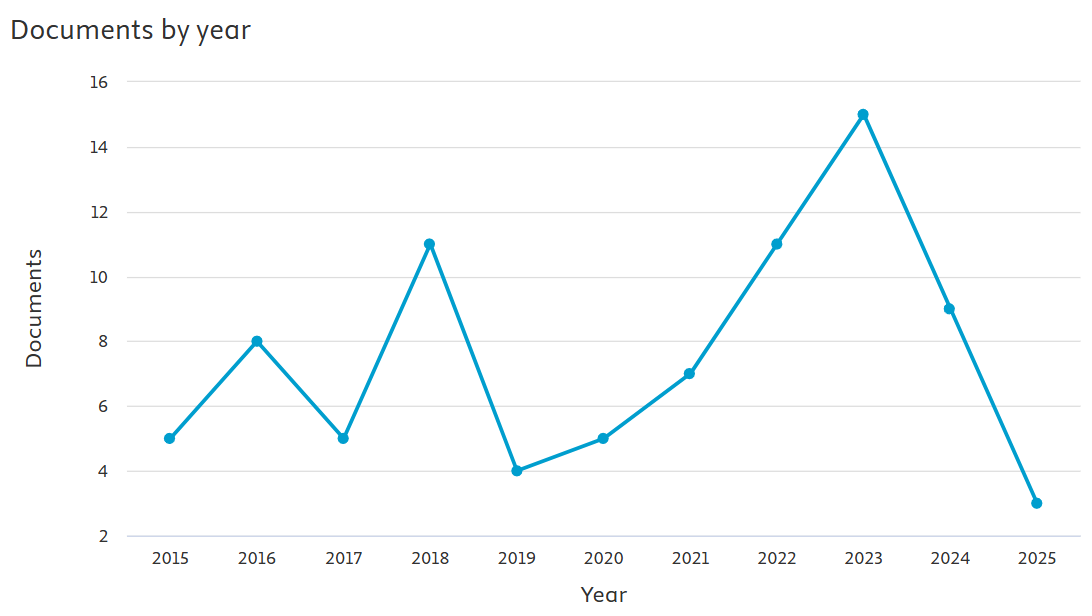
\includegraphics[width=0.9\textwidth]{media/docs_by_year.png}
    \legend{Fonte: Scopus}
    \label{fig:docs_by_year}
\end{figure}

Na \autoref{fig:docs_by_country} são apresentados os países com maior número de publicações relacionadas ao tema desta pesquisa. Observa-se que a China lidera com 10 documentos, seguida pela Alemanha (7) e pelos Estados Unidos (6). Em seguida, aparecem Índia, Reino Unido e Suíça, cada um com 5 documentos publicados. A Turquia também se destaca com 4 publicações, enquanto Croácia, Estônia e França completam a lista com 2 documentos cada. Esses dados evidenciam uma concentração relevante de estudos em países com infraestrutura tecnológica consolidada, especialmente na Ásia, Europa Ocidental e América do Norte, o que reforça o caráter global do interesse em torno da comparação entre abordagens de renderização no desenvolvimento de aplicações web.

\begin{figure}[H]
    \centering
    \caption{Distribuição das publicações por país}
    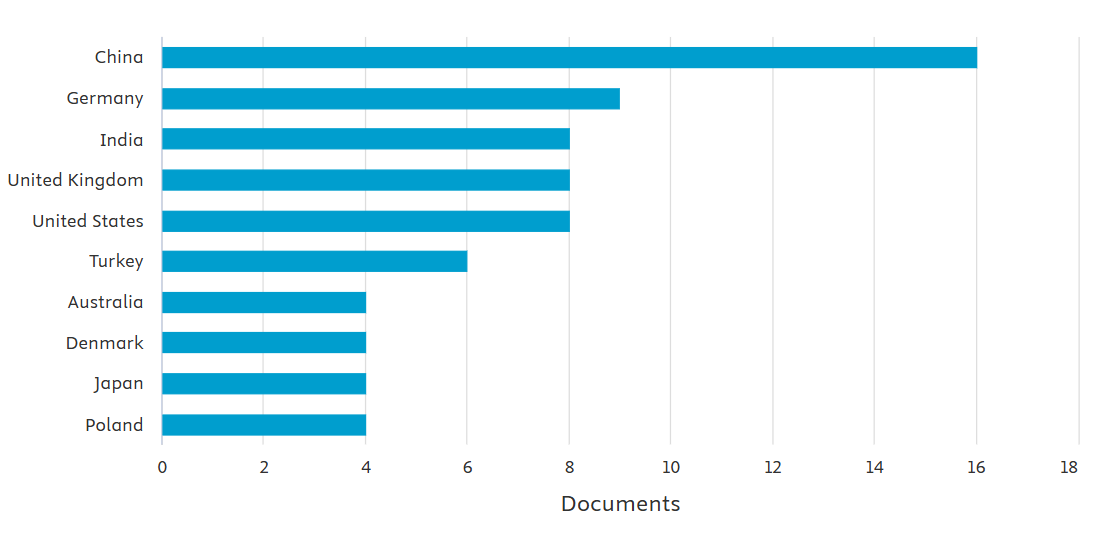
\includegraphics[width=0.9\textwidth]{media/docs_by_country.png}
    \legend{Fonte: Scopus}
    \label{fig:docs_by_country}
\end{figure}


\section{Artigos selecionados}
\label{section:artigos_selecionados}

Após realizadas as leituras preliminares, apenas 13 publicações mostraram-se relevantes para responder às questões de pesquisa e/ou apoiar na elaboração do estudo de caso. Esta seleção considerou critérios de alinhamento temático, profundidade técnica e aplicabilidade ao escopo da pesquisa. A listagem completa dos artigos selecionados pode ser consultada no Quadro~\ref{quad:publicacoes_desenvolvimento_web}.

\begin{quadro}[H]
    \centering
    
    \setlength{\tabcolsep}{0.8em} % espaçamento horizontal
    \renewcommand{\arraystretch}{1.5}% espaçamento vertical
    \begin{tabular}{p{4in}|p{0.5in}}
    \hline
    
    \multicolumn{1}{|p{4in}}{\textbf{Título}} & 
    \multicolumn{1}{|p{0.5in}|}{\textbf{Ano}} \\
    \hhline{--}
    
    \multicolumn{1}{|p{4in}}{\english{Progressive Server-Side Rendering with Suspendable Web Templates}} & 
    \multicolumn{1}{|p{0.5in}|}{\citeyear{Carvalho2025458}} \\
    \hhline{--}
    
    \multicolumn{1}{|p{4in}}{\english{Requirements for the Development of a Website Builder with Adaptive Design}} & 
    \multicolumn{1}{|p{0.5in}|}{\citeyear{Bekmanova2024265}} \\
    \hhline{--}
    
    \multicolumn{1}{|p{4in}}{\english{Enhancing SEO in Single-Page Web Applications in Contrast With Multi-Page Applications}} & 
    \multicolumn{1}{|p{0.5in}|}{\citeyear{Kowalczyk202411597}} \\
    \hhline{--}
    
    \multicolumn{1}{|p{4in}}{\english{Web Development Using ReactJS}} & 
    \multicolumn{1}{|p{0.5in}|}{\citeyear{Keshari20231571}} \\
    \hhline{--}
    
    \multicolumn{1}{|p{4in}}{\english{Improving Universal Rendering Performance on NuxtJS-based Web Application}} & 
    \multicolumn{1}{|p{0.5in}|}{\citeyear{Angkasa2023}} \\
    \hhline{--}
    
    \multicolumn{1}{|p{4in}}{\english{Comparison between client-side and server-side rendering in the web development}} & 
    \multicolumn{1}{|p{0.5in}|}{\citeyear{FadhilahIskandar2020}} \\
    \hhline{--}
    
    \multicolumn{1}{|p{4in}}{\english{Methods of Improving and Optimizing React Web-applications}} & 
    \multicolumn{1}{|p{0.5in}|}{\citeyear{Pavic20211753}} \\
    \hhline{--}
    
    \multicolumn{1}{|p{4in}}{\english{Improving ruby on rails-based web application performance}} & 
    \multicolumn{1}{|p{0.5in}|}{\citeyear{Klochkov2021}} \\
    \hhline{--}
    
    \multicolumn{1}{|p{4in}}{\english{An integrated framework of user experience-oriented smart service requirement analysis for smart product service system development}} & 
    \multicolumn{1}{|p{0.5in}|}{\citeyear{Zhou2022}} \\
    \hhline{--}
    
    \multicolumn{1}{|p{4in}}{\english{A Research Framework for B2B Green Marketing Innovation: the Design of Sustainable Websites}} & 
    \multicolumn{1}{|p{0.5in}|}{\citeyear{Lacom2022}} \\
    \hhline{--}
    
    \multicolumn{1}{|p{4in}}{\english{Corporate Social Responsibility: Hiring Requisition in Media Companies?}} & 
    \multicolumn{1}{|p{0.5in}|}{\citeyear{Boehncke202375}} \\
    \hhline{--}
    
    \multicolumn{1}{|p{4in}}{\english{Single page optimization techniques using react}} & 
    \multicolumn{1}{|p{0.5in}|}{\citeyear{Pokhriyal2024338}} \\
    \hhline{--}

    \multicolumn{1}{|p{4in}}{\english{Proceedings of the 19th International Conference on Web Information Systems and Technologies, WEBIST 2023}} & 
    \multicolumn{1}{|p{0.5in}|}{\citeyear{2023}} \\
    \hhline{--}
    
    \end{tabular}
    \caption{Artigos selecionados sobre estratégias de renderização e desempenho em aplicações web}
    \label{quad:publicacoes_desenvolvimento_web}
\end{quadro}
    

\section{Resultados e Discussão}
\label{section:resultados_discussao}


% https://www-scopus-com.ez135.periodicos.capes.gov.br/results/results.uri?sort=plf-f&src=s&sid=c5e620a132b74a852dccc08c5c330e9d&sot=a&sdt=cl&sl=247&s=%28TITLE-ABS-KEY%28%22Client-Side+Rendering%22+OR+%22CSR%22+OR+%22Server-Side+Rendering%22+OR+%22SSR%22%29%29+AND+%28TITLE-ABS-KEY%28%22web+performance%22+OR+%22page+speed%22+OR+%22web+optimization%22+OR+%22SEO%22+OR+%22search+engine+optimization%22+OR+%22user+experience%22+OR+%22UX%22+OR+%22usability%22%29%29&origin=resultslist&editSaveSearch=&txGid=584773b92f904689225d6d8bd0143429&sessionSearchId=c5e620a132b74a852dccc08c5c330e9d&limit=10&yearFrom=2020&yearTo=2025
